\documentclass[a4paper,10pt]{article}
\usepackage[a4paper, total={6in, 10in}]{geometry}
\setlength\parindent{0pt}
\usepackage[utf8]{inputenc}
\usepackage{graphicx} 
\usepackage{amsmath}
\usepackage{amsfonts}
\usepackage{amssymb}
\usepackage{listings}
\usepackage{ragged2e}
\usepackage{listings}
\usepackage{color}
\usepackage[table]{xcolor}
\usepackage{soul}
\usepackage[font=small,labelfont=bf]{caption}
\setlength{\parskip}{\baselineskip}%
\setlength{\parindent}{0pt}%

\begin{document}
\begin{titlepage}
	\centering
	
\includegraphics[width=.6\textwidth]{liu-logo.png}\par
	\vfill
	{\scshape\Large TDDD41 Data Mining - Clustering and Association Analysis\par}
	{\huge\bfseries Lab 3 -  Group 4 Report\par}
	\vspace{0.5cm}
    {\large\itshape Lawrence Thanakumar Rajappa (lawra776)\\
     \large\itshape Kyriakos Domanos (kyrdo817)\par}
	\vfill
	{\large \today\par}
\end{titlepage}
\definecolor{dkgreen}{rgb}{0,0.6,0}
\definecolor{gray}{rgb}{0.5,0.5,0.5}
\definecolor{mauve}{rgb}{0.58,0,0.82}

\begin{center}
	\large\textbf{\underline{Association Analysis-2}} \par
\end{center} \par
\textbf{\underline{Data Preparation}} \par
In this lab assignment, we used Monk1 dataset which contains 124 samples of data, 7 attributes and target 
variable is binary. As a starting process, we checked whether the data contains continuous format, but all
attributes were discrete.  \par
\textbf{\underline{Clustering}} \par
Now, we tried to apply \textbf{\textit{SimpleKmeans}} clustering algorithm with the following specifications;
\begin{enumerate}
  \item[$*$] \textbf{Seed value} $:$ 10
  \item[$*$] \textbf{No. of Clusters} $:$ 2 
\end{enumerate}
and igonred \textbf{\textit{class}} attribute and selected Classes to clusters evaluation to crosstabulate the 
clustering. We have got 47.5806\% incorrectly clustered instances. When we tried with \textbf{\textit{MakeDensity
BasedClusterer}} with the default parameters, we got 45.9677\% which was not a good improvement.
\par
\textbf{Why can the clustering algorithm not find a division that matches the class division in the database?} \par
When visualizing the results of cluster, we could see that there is overlapping of data points and moreover,
there is not well-defined boundary, this makes the separation tedious. In order to have a proper separation,
similar data points should lie close to each other, this would make the jobs of clustering algorithm easy.
In order to have a proper clustering, we could either use \textbf{\textit{overlapping clustering}} technique
or preprocess the data by adding some more attributes to the data which could increase the chances of separation.
\begin{center}
  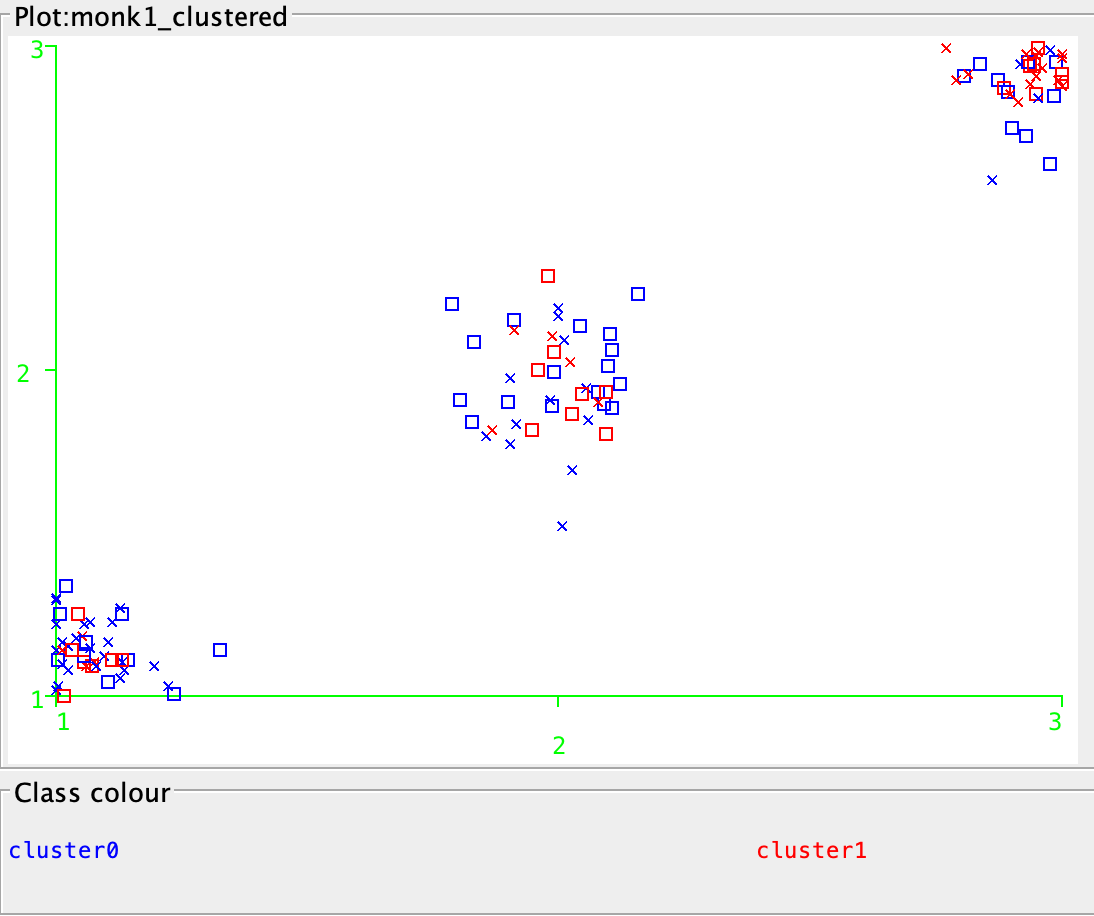
\includegraphics[width=80mm,scale=0.10]{Clustering_Visualization.png}
  \captionof{figure}{Overlapping data points}
\end{center}
\par
\textbf{Would you say that it goes poorly for monk1? Why or why not?} \par
From the data, we could conclude that the results of clustering algorithms were bad are because of
characteristics of the data. As said earlier, if we provide the preprocessed data to the algorithms,
we could get a better result and performance. But there is another way to handle this, i.e. we need 
to create a new distance function which can be incorporated into the existing algorithms to create
a separation for this type of data, but on the other hand, it requires lot of expertise and knowledge
for a domain for the data related to that domain.
\par
\textbf{\underline{Association Analysis - Apriori}} \par
Here we have used the following specifications for performing Apriori algorithm on 3 clustered dataset;
\begin{enumerate}
  \item [$*$] \textbf{Minimum Support} = 0.1
  \item [$*$] \textbf{Metric type} = Confidence
  \item [$*$] \textbf{Minimum Confidence} = 0.9
\end{enumerate}
with the above properties, we have performed apriori algorithm on the iris dataset and got the following association rules
which are given below,

In this frequent itemset are the attribute-value pair and transaction is a single data point. Moreover, with 
default properties we weren't able to get proper association rules, hence we changed our properties a bit;
\begin{enumerate}
  \item [$*$] \textbf{Number of Rules} = 1000
  \item [$*$] \textbf{Metric type} = Confidence
  \item [$*$] \textbf{Minimum Confidence} = 0.9
\end{enumerate}
In the above properties, \textbf{\textit{Number of Rules}} which specifies how many rules are needed and we get
1000 rules from this property and we keep the rule with 90\% confidence.
\begin{enumerate}     
  \item [$*$] sepalwidth='(-inf-2.8]' petallength='(2.966667-4.933333]' ==$>$ Cluster=cluster1, Occurrence = 30, Confidence:(1)
  \item [$*$] petallength='(2.966667-4.933333]' petalwidth='(0.9-1.7]' ==$>$ Cluster=cluster1, Occurrence = 48, Confidence:(1)
  \item [$*$] petallength='(4.933333-inf)' petalwidth='(1.7-inf)' ==$>$ Cluster=cluster2, Occurrence = 40, Confidence:(1)
  \item [$*$] sepallength='(6.7-inf)' petallength='(4.933333-inf)' ==$>$ Cluster=cluster2, Occurrence = 17, Confidence:(1)
  \item [$*$] sepallength='(-inf-5.5]' petallength='(-inf-2.966667]' ==$>$ Cluster = cluster3, Occurrence = 47, confidence:(1)
  \item [$*$] sepalwidth='(2.8-3.6]' petallength='(-inf-2.966667]' ==$>$ Cluster=cluster3, Occurrence = 36, Confidence:(1)
\end{enumerate}
\par
From the above association rules, we could see that we want class to be in consequent rather than in antecedent, because
we need to predict the class of the flower and also when a new data comes into the system, we need to predict its species
instead of having the class at beginning and attributes are placed in consequent because it is not to be predicted. \par
\textbf{\underline{Experiments}} \par
\textbf{\underline{Different Number of Bins}} \par
By increasing number of bins, we could yield more information and thus we can calculate distance between data points 
more precisely in k-means algorithm. On the other hand, having to many clusters which would yield less information and
possibly it could make the algorithm ambiguous. 

We tried to discretize the data with \textbf{\textit{6 bins}} and found that the amount of incorrectly clustered
data points are more when compared with the clustering result with 3 bins, which makes the above line true. We then
applied \textbf{\textit{addCluster}} filter on the 6 bins data and found the following association rules;
\begin{enumerate}
  \item [$*$] petallength='(-inf-1.983333]' ==$>$ cluster=cluster1, occurrence = 50    conf:(1)
  \item [$*$] petalwidth='(-inf-0.5]' ==$>$ cluster=cluster1, occurrence = 49    conf:(1)
  \item [$*$] sepallength='(5.5-6.1]' petallength='(3.95-4.933333]' ==$>$ cluster=cluster2, occurrence = 21    conf:(1)
  \item [$*$] petallength='(3.95-4.933333]' petalwidth='(0.9-1.3]' ==$>$ cluster=cluster2, occurrence = 18    conf:(1)
  \item [$*$] sepallength='(6.1-6.7]' petallength='(4.933333-5.916667]' ==$>$ cluster=cluster3, occurrence = 20    conf:(1)
  \item [$*$] sepalwidth='(2.8-3.2]' petallength='(4.933333-5.916667]' ==$>$ cluster=cluster3, occurrence = 18    conf:(1)
\end{enumerate}
From the association rules above, we infer that cluster1 is characterized by only petal length and petal width, while
cluster2 and cluster3 are characterized by mix of attribute values. This clustering is not good because there is 20.6667\% 
of incorrectly clustered instances. This is because some of the values don't reach the minimum support and don't
give rise to correct rules. From this we can conclude that instead of increasing the bins, we can perform discretize
in an efficient way.
\par
\textbf{\underline{Different Number of Clustering Algorithms}} \par
We started with \textbf{\textit{Hierarchical Clustering}} with 3 binned data, and got the below confusion matrix and 
incorrect clustered instance;

When compared Hierarchical clustering with SimpleKmeans, we could see that there is an increase in the percentage
of incorrectly clustered data points. In theory, Hierarchical clustering works by creating clusters for \textbf{N}
datapoints, so we will have \textbf{N} clusters and then combine them based on similarity measure. The similarity 
between the clusters is often calculated from the dissimilarity measures like the euclidean distance between two 
clusters. So the larger the distance between clusters, the better it is. So the reason for bad performance
could be distance between clusters would have been lesser, hence data points were not clustered properly.
\par
Then we started with \textbf{\textit{Filtered Clustering}}, we could see that results were same as the results of
SimpleKmeans algorithm and there was a swap of datapoints between clusters for species Iris-virginica and Iris-versicolor,
but Iris setosa was clustered properly.

\par
\textbf{\underline{Different Number of Clusters}} \par
From the dataset, we could see that it has only 3 classes, hence we can have 3 clusters. But, if we want to have 
more than the specified number of clusters, there is going to be further subdivision or partition in the data and 
some data points are going to be assigned to clusters which have no class names.
\newpage
We started our experiment with 6 clusters, and found the following results;

We performed Apriori algorithm on data with 6 clusters and found association rules only for clusters 0,1, and 4
and not for clusters 2,3 and 5 with \textit{numrules} = 50 ,despite giving minimum confidence. Also, we could see that incorrectly clustered 
data points are more with 6 clusters because minimum confidence was not attained as well as some points of same 
class belongs to the larger clusters. From this information, we can infer that it is better to use 3 class 
partition to separate the data points very accurately.
\end{document}